\documentclass{article}

% The following \documentclass options may be useful:

% preprint      Remove this option only once the paper is in final form.
% 10pt          To set in 10-point type instead of 9-point.
% 11pt          To set in 11-point type instead of 9-point.
% authoryear    To obtain author/year citation style instead of numeric.

\usepackage[dvipsnames]{xcolor}
\usepackage{siunitx}
\usepackage{amsmath}
\usepackage{amsfonts}
\usepackage{amssymb}
\usepackage{array}
\newcolumntype{L}[1]{>{\raggedright\let\newline\\\arraybackslash\hspace{0pt}}m{#1}}
\newcolumntype{C}[1]{>{\centering\let\newline\\\arraybackslash\hspace{0pt}}m{#1}}
\newcolumntype{R}[1]{>{\raggedleft\let\newline\\\arraybackslash\hspace{0pt}}m{#1}}
\usepackage[utf8]{inputenc}
\usepackage[english]{babel}
\usepackage{pgfplots}
\usepackage{url}
\usepackage{hyperref} 
\usepackage{float}
\usepackage{tabularx,caption}
\usepackage{csvsimple}
\usepackage{listings,mdframed}

\lstset{
	language=java,
	keywordstyle=\bfseries\ttfamily\color[rgb]{0,0,1},
	identifierstyle=\ttfamily,
	commentstyle=\color[rgb]{0.133,0.545,0.133},
	stringstyle=\ttfamily\color[rgb]{0.627,0.126,0.941},
	showstringspaces=false,
	basicstyle=\small,
numberstyle=\tiny,
numbers=right,
	stepnumber=1,
	numbersep=10pt,
	tabsize=1,
	breaklines=true,
	prebreak = \raisebox{0ex}[0ex][0ex]{\ensuremath{\hookleftarrow}},
	breakatwhitespace=false,
	aboveskip={1.5\baselineskip},
  columns=fixed,
  upquote=true,
  extendedchars=true,
 frame=single,
 inputencoding=utf8,
    literate={á}{{\'a}}1 {ã}{{\~a}}1 {â}{{\~a}}1 {é}{{\'e}}1 {ê}{{\'e}}1 {ç}{{\'c}}1 {ú}{{\'u}}1 {ó}{{\'o}}1 {í}{{\'i}}1,
 %backgroundcolor=\color{lbcolor},
}

\hypersetup{colorlinks =false}

\begin{document}

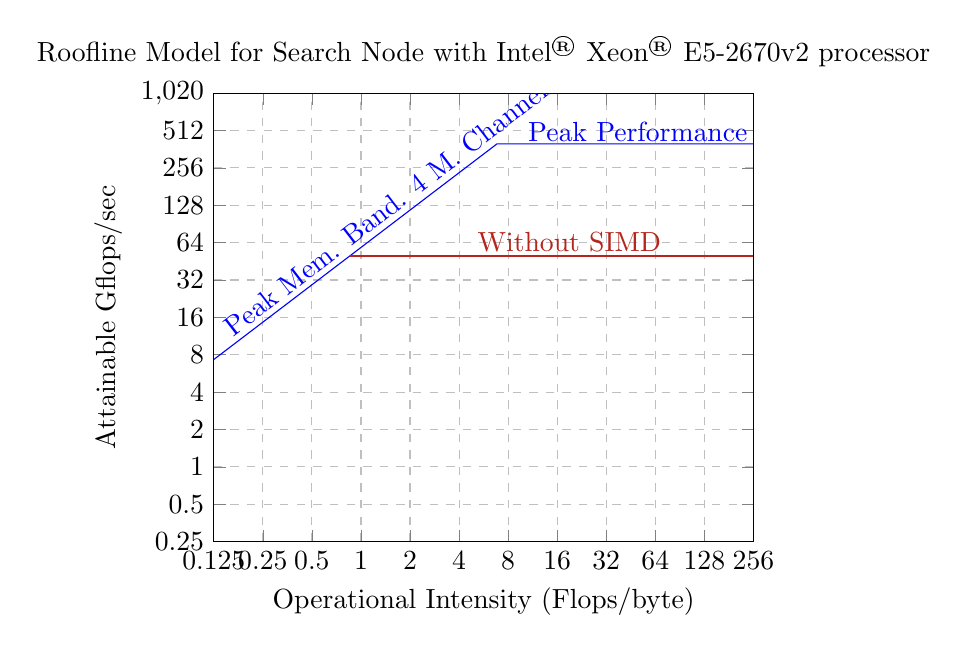
\begin{tikzpicture}
  \label{fig:roofline_team}

\begin{axis}[
    title={Roofline Model for Search Node with Intel\textsuperscript{\textregistered} Xeon\textsuperscript{\textregistered} E5-2670v2 processor},
    xlabel={Operational Intensity (Flops/byte)},
    ylabel={Attainable Gflops/sec},
    xmin=0.125, xmax=256,
    ymin=0.25, ymax=1024,
    xtick={0.125,0.25,0.5,1,2,4,8,16,32,64,128,256},
    ytick={0.25,0.5,1,2,4,8,16,32,64,128,256,512,1024},
    legend pos=north west,
    ymajorgrids=true,
    xmajorgrids=true,
    grid style=dashed,
    xmode=log,
    ymode=log,
    log ticks with fixed point
]
 
\addplot[
    color=blue,
    ]
    coordinates {
    (0.125,7.318625)(6.83188,400)(256,400)
    };
    \node[rotate=37.5,text=blue] at (axis cs: 1.5,128) {Peak Mem. Band. 4 M. Channels};
    
\node [above,text=blue] at (axis cs: 50,350) {Peak Performance};



    
\addplot[
    color=BrickRed,
    ]
    coordinates{
    (0.853985,50)(256,50)
    };
\node [above,text=BrickRed] at (axis cs: 19,45) {Without SIMD};

\end{axis}

\end{tikzpicture}

\end{document}